\section{Electromagnetism in Special Relativity}
\subsection{Potential Four Vector}
\subsection*{Vector Potential}
Before we discuss how the relativistic electric and magnetic fields, we need to define a useful vector field called the \textit{vector potential}. Recall that one of Maxwell's equations is \begin {equation} \oiint \vec{B} \cdot d\vec{S} = 0 \label{eq:nomagmon} \end{equation} because there are no magnetic monopoles. This means that $\vec{B}$ is solenoidal, so we can define a vector field $\vec{A}$ such that  \begin{equation} \nabla\times\vec{A} = \vec{B}. \label {eq:A} \end{equation} $\vec{A}$ is the vector potential. Note that it is not unique, as adding any conservative vector field to $\vec{A}$ will yield another solution to Eq. \ref{eq:A}.

Recall also that 
\begin{equation} \oint \vec{E} \cdot d\vec{\ell} = - \frac{d}{dt} \oiint \vec{B} \cdot d\vec{S}. \label{eq:faraday-lenz} \end{equation}
By Stokes' theorem,
$$\oiint \vec{B} \cdot d\vec{S} = \oiint (\nabla \times \vec{A}) \cdot d\vec{S} = \oint \vec{A} \cdot d\vec{\ell},$$ so 

$$\oint \left(\vec{E} +\frac{d \vec{A}}{dt}\right) \cdot d \vec{\ell} = 0.$$ This allows us to define a \textit{scalar potential} $\phi$ such that 
\begin{equation}-\nabla \cdot \phi = \vec{E} +\frac{d \vec{A}}{dt}.\label{eq:scalpot}\end{equation} This is the generalization of the electric potential you learned about in AP Physics to the case where there's a time-dependent magnetic field present.
\subsection*{4-Potential}
Now, let's do a simple example to understand how $\vec{E}$ and $\vec{B}$ transform in special relativity. Suppose in our lab frame we have an infinite line of stationary charge with density $\lambda$. Clearly, since there are no charges in motion in this frame, we have 
\begin{equation}\vec{B} = 0 \label{eq:Blab}.\end{equation}

To calculate the electric field in this frame, we use the cylindrical Gaussian surface depicted in figure \ref{1}.
\begin{figure}[ht]
\centering
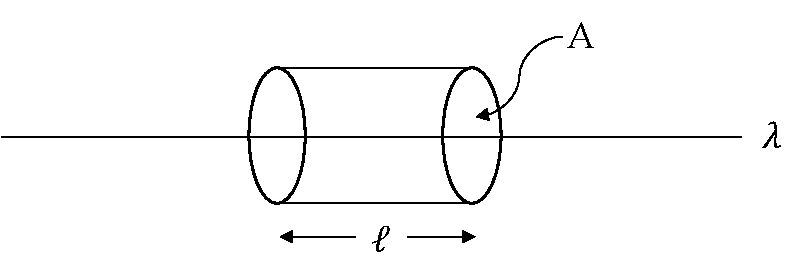
\includegraphics[width=7cm]{images/relativity/surface.pdf}
\caption {Gaussian surface for analysis of infinite line charge}
 \label{1}
\end{figure} 
 The electric field is obviously radial by symmetry. Suppose the surface has radius $r$. The flux through the cylinder is then $E 2 \pi r \ell $ and the charge is $\ell \lambda$, so \[\vec{E} = \frac{\lambda}{2\pi\epsilon_0 r} \hat{e}_r. \]
Because $\vec{B} = 0$, we can choose $\vec{A} = 0$. Then clearly \[ \phi = -\frac{\lambda}{2\pi \epsilon_0} \ln r.\]

Now let us consider a frame in which the charge is moving to the right at speed $v$. The charge density is now $\gamma \lambda$ because lengths have been contracted by a factor of $\gamma$.

There is now a nonzero magnetic field. We apply Ampere's Law to find it. We use a loop of radius $r$ whose central axis coincides with the wire. Ampere's Law gives $2 \pi r B = \mu_0 I$. In a time interval $dt$, charge $\gamma \lambda v dt$ will move past a certain point, so $I = \gamma \lambda v$. Therefore \[\vec{B} = \frac{\gamma\mu_0\lambda v}{2\pi r} \hat{e}_\theta. \] 
Also, 
\[\vec{E} = \frac{\gamma \lambda}{2\pi\epsilon_0 r} \hat{e}_r. \]

We need the curl of the vector potential to only have a nonzero component along 
$\hat{e}_\theta$. The component of the curl is \[\frac{\partial A_r}{\partial z} - \frac{\partial A_z}{\partial r} .\] We choose $\vec{A}$ to be purely in the $z$-direction, so \[\vec{A} = -\frac{\mu_0 \gamma \lambda v}{2\pi} \ln r \hat{k} .\] Since the magnetic field is not time-dependent, 
\[\phi = -\frac{\gamma \lambda}{2\pi\epsilon_0} \ln r .\]

Notice that the transformation from one reference frame to another is exactly the Lorentz transformation:
\[
\Lambda \begin{pmatrix} \frac{\phi}{c} \\ 0 \end{pmatrix} = \begin{pmatrix}
\gamma \frac{\phi}{c} \\
\gamma \frac{v}{c^2} \phi 
\end{pmatrix} = \begin{pmatrix}
-\frac{\gamma \lambda}{2\pi\epsilon_0c} \ln r \\ -\frac{\gamma\lambda v}{2\pi \epsilon_0 c^2 r} \ln r
\end{pmatrix} = \begin{pmatrix}
-\frac{\gamma \lambda}{2\pi\epsilon_0c} \ln r \\ -\frac{\gamma\lambda v\mu_0}{2\pi  r} \ln r
\end{pmatrix}.
\]
This suggests that we define a new four-vector: the \textbf{four-potential} $A^\mu = (\phi/c, \vec{A}) $. 
\subsection{Field Strength Tensor}
We're now going to define the \textbf{field strength tensor}. Before that, though, we have to understand how derivatives transform. We have 
\begin{equation*}
    \frac{\partial}{\partial x'^{\mu}} = \frac{\partial x^{\nu}}{\partial x'^{\mu}} = (\Lambda^{-1})_\mu^\nu \frac{\partial}{\partial x^\nu}.
\end{equation*}
This is the opposite of how the position 4-vector transforms:
\begin{equation*}
    x'^{\mu} = \Lambda_{\nu}^{\mu} x^{\nu}.
\end{equation*} We say that the position 4-vector transforms contravariantly, while the derivative is covariant. The familiar derivative is written with a lower index, unlike the position, which is written with an upper index. 

We now define the field strength tensor:
\begin{equation}
    F^{\mu \nu} = \partial^\mu A^\mu - d^\nu A^\mu.
\end{equation}
We can calculate a few components:
\begin{align*}
    F^{01} &= \partial^0 A^1 - \partial^1 A^0 = \frac{\partial A_x}{c\partial t} + \frac{\partial(\phi/c)}{\partial x} = -\frac{E_x}{c}, \\
        F^{30} &= \partial^3 A^0 - \partial^0 A^3 = -\frac{\partial (\phi/c)}{\partial z} - \frac{\partial A_z}{c\partial t} = \frac{E_z}{c},\\
        F^{12} &= \partial^1 A^2 - \partial^2 A^1 = -\frac{\partial A_y}{\partial x} + \frac{\partial A_x}{\partial y} = -B_z,\\
        F^{23} &= \partial^2 A^3 - \partial^3 A^2 = -\frac{\partial A_z}{\partial y} + \frac{\partial A_y}{\partial z} = -B_x.\\
\end{align*}
The rest of the components can be calculated in an analogous manner. The entire field strength tensor is then 
\begin{equation}
    F^{\mu\nu} = \begin{pmatrix}
    0 & -\frac{E_x}{c} & -\frac{E_y}{c} & -\frac{E_z}{c} \\
    \frac{E_x}{c} & 0 & -B_z & B_y \\
    \frac{E_y}{c} & B_z & 0 & -B_x \\
    \frac{E_z}{c} & -B_y & B_x & 0
    \end{pmatrix}.
\end{equation}
\subsection{Transformations of Electric and Magnetic Fields}
We can use the field strength tensor to transform the electric and magnetic fields. We can transform between frames using the Lorentz transformation:
\[F'^{\mu \nu} = \Lambda_{\alpha}^{\mu} \Lambda_{\beta}^{\nu} F^{\alpha \beta}. \]

For example, if we boost in the $x$-direction, we have
\begin{align*}
    \frac{E_x'}{c} &= F'^{10} = \Lambda_\alpha^1 \Lambda_\beta^0 F^{\alpha \beta} = \Lambda_0^1 \Lambda_1^0 F^{01}+\Lambda_1^1 \Lambda_0^0 F^{10} = \gamma^2 \frac{v^2}{c^2} \left(-\frac{E_x}{c}\right) + \gamma^2 \frac{E_x}{c} = \frac{E_x}{c},\\
    \frac{E_y'}{c} &= F'^{20} = \Lambda_\alpha^2 \Lambda_\beta^0 F^{\alpha \beta} = \Lambda_{2}^{2} \Lambda_1^0 F^{21} + \Lambda_2^2 \Lambda_0^0 F^{20} = \gamma \frac{v}{c} B_z + \gamma \frac{E_y}{c},\\
    B_x' &= F'^{32} = \Lambda_\alpha^3 \Lambda_\beta^2 F^{\alpha \beta} = B_x,\\
    B_y' &= F'^{31} = \Lambda^3_\alpha \Lambda^1_\beta F^{\alpha \beta} = \Lambda_0^1 F^{30} +\Lambda_1^1 F^{31} = \frac{\gamma v}{c} \left(-\frac{E_z}{c}\right)+\gamma B_y = \gamma\left(B_y-\frac{v}{c^2} E_z \right).
\end{align*}
In general, we can see that 
\begin{align*}
    \vec{E}_\parallel' &= \vec{E}_\parallel,\\ \vec{E}_\perp' &= \gamma( \vec{E}_\perp-\vec{v} \times \vec{B}), \\
    \vec{B}_\parallel' &= \vec{B}_\parallel, \\
    \vec{B}_\perp' &= \gamma\left( \vec{B}_\perp+\frac{1}{c^2}\vec{v} \times \vec{E}\right).
\end{align*}
\subsection{Invariants}
Two important invariants are 
\begin{align*}
    F^{\mu\nu} F_{\mu \nu} = 2|\vec{B}|^2 - \frac{2|\vec{E}|^2}{c^2} &\propto E^2-c^2B^2 \\
    \epsilon_{\mu\nu\alpha\beta} F^{\mu\nu} F^{\alpha\beta} &\propto \frac{\vec{E}\cdot\vec{B}}{c}.
\end{align*}